% Hand-written text; every number is a macro from generated/numbers.tex (paper/make_numbers.py).
\section{Confirmatory results}\label{sec:results}

\subsection{Execution and validity}
All \GridValid{} of \GridRuns{} registered runs (48 configurations $\times$ 2 seeds, Slurm array 4036, one commit, two runs at a time on two L40 GPUs) completed and passed every validation check: run status and final step, learning rate, seed, horizon and evaluation cadence, the SHA-256 of each verifier configuration against its registered file, the $\qref$ lock hash, a clean source tree, the evaluation schedule, and a complete verifier decision log. The digest of the configuration directory equals the value committed in the registration. No run was rerun, excluded or replaced, and no run diverged (\Divergences{} runs met the registered divergence definition). Training used \GPUhours{} GPU-hours at a median of \StepSecMed{}~s per step.

\textbf{Realised verifier rates.} The verifier logs record every decision. The realised acceptance rate of correct rollouts was between \TaurealMin{} and \TaurealMax{} in every run, matching $\tau=0.9$. Over all training steps, the realised false-acceptance rate on wrong rollouts in the matched arm averaged \FrealAllMatched{}, against the design value 0.3 under $\qref$; in the outcome window it ranged from \FrealMatchedMin{} to \FrealMatchedMax{} across runs (mean \FrealMatchedMean). This spread is expected: $\Fbar$ is matched under the \emph{base} error distribution, and the policy's error distribution moves during training (Proposition~2). The window rate is rank-correlated with $V$ (Spearman \SpearFrealV), so it is a post-treatment quantity, not a covariate.

\textbf{Disclosure: duplicated verifier configurations.} After the registered analysis was run, we found that the registered grid contains exact duplicates. The generator drew three candidates per grid cell, and in several cells the constraints fix the acceptance vector up to the choice of mode, so some candidates coincide; for example, every $V$-fraction-0 cell yields the homogeneous verifier. The 36 matched configurations contain \NuniqueMatched{} distinct verifiers (\NdupGroups{} groups of duplicates), and the 48 configurations contain \NuniqueAll. Because a run is a deterministic function of the verifier, the seed and the evaluation cadence, duplicated configurations produced bit-identical outcomes. Two consequences matter: the registered H1 treats 36 rows as independent when 25 are distinct, which understates its standard error; and \NheldTwin{} of the \NheldOut{} held-out configurations have an identical twin among the training configurations, so part of the registered held-out comparison is not out-of-configuration. The registered analysis is reported unchanged below. Each primary quantity is then re-estimated on distinct verifiers only, as a sensitivity analysis labelled exploratory (Section~\ref{sec:robust}).

\subsection{Registered estimates}

\begin{table}[t]
\centering
\caption{Registered primary estimates (matched arm, configuration = unit). The registration declared these estimates with confidence intervals as the primary results; $p$-values are reported but not interpreted as confirmatory tests (power was below 0.5). MSE differences are paired, negative values favour the first predictor set.}
\label{tab:primary}
\small
\begin{tabular}{@{}llll@{}}
\toprule
Quantity & Estimate & 95\% CI & $p$ (Holm) \\
\midrule
H1: $b_V$ (HC3, $n=36$, df 33) & \HoneBV & [\HoneLo, \HoneHi] & \HoneP{} (\HolmHone) \\
H1: $b_f$ (same fit) & \HoneBF & [\HoneBFLo, \HoneBFHi] & -- \\
H2: MSE$\{\fmax,V\}$ $-$ MSE$\{\fmax\}$, 13 held out & \HtwoDiff & [\HtwoLo, \HtwoHi] & \HtwoP{} (\HolmHtwo) \\
H3: MSE$\{Z(s)\}$ $-$ MSE$\{\fmax,V\}$, $s=\HthreeS$ & \HthreeDiff & [\HthreeLo, \HthreeHi] & \HthreeP{} (\HolmHthree) \\
\midrule
\multicolumn{4}{@{}l}{\emph{Sensitivity, distinct verifiers only (exploratory)}}\\
H1: $b_V$ ($n=\NuniqueMatched$, df 22) & \UniqBV & [\UniqBVLo, \UniqBVHi] & -- \\
H1: $b_f$ & \UniqBF & [\UniqBFLo, \UniqBFHi] & -- \\
Leave-one-verifier-out: $\{\fmax,V\}-\{\fmax\}$ & \UniqDiff & [\UniqDiffLo, \UniqDiffHi] & \UniqDiffP \\
Leave-one-verifier-out: $\{Z(s)\}-\{\fmax,V\}$ & \UniqZDiff & [\UniqZDiffLo, \UniqZDiffHi] & -- \\
Held out without twins ($n=\PureN$): H2 difference & \PureDiff & [\PureLo, \PureHi] & -- \\
\bottomrule
\end{tabular}
\end{table}

\textbf{H1 (dispersion at matched rates).} Across the 36 matched configurations, $\bar Y$ decreased with $V$ at fixed $\fmax$: $b_V=\HoneBV$ logit per unit of $V$ (HC3 95\% CI \HoneLo{} to \HoneHi; Table~\ref{tab:primary}, Figure~\ref{fig:h1}). Over the realised range of $V$ (0 to about 0.17), this corresponds to roughly one logit unit of window accuracy. The fit explains $R^2=\HoneRsq$ of the between-configuration variance, and the rank correlation of $\bar Y$ with $V$ is \SpearmanYV. With $V$ in the model, the worst-mode rate has a small positive coefficient ($b_f=\HoneBF$, CI \HoneBFLo{} to \HoneBFHi), which does not survive deduplication. The point estimate is close to the planning value used for the power analysis ($b_V=\PlanBV$), but the interval is much narrower than that analysis anticipated. The power simulation set the between-configuration SD to the pilot's seed SD (\SigmaS) as a conservative floor and added seed noise on top. In the grid, seed noise is heavy-tailed: most seed pairs differ by little (median gap \SeedGapMed{} logit), while a few high-$V$ pairs differ by more than one logit (Section~\ref{sec:results}, mechanism), so the one-way ICC is only \ICCmatched{} even though $V$ and $\fmax$ explain most of the between-configuration variance. The precision of $b_V$ is a property of this grid and should not be read as evidence that the planning noise model was wrong in general.

\textbf{H2 (held-out prediction beyond $\fmax$).} Fitted on the 23 training configurations, $\{\fmax,V\}$ predicted the 13 held-out configurations with MSE \HtwoMSEfv, against \HtwoMSEf{} for $\fmax$ alone (difference \HtwoDiff, CI \HtwoLo{} to \HtwoHi; Holm-adjusted $p$ \HolmHtwo; Figure~\ref{fig:heldout}). Leave-one-configuration-out MSE on all matched configurations agrees (\LocoFV{} vs \LocoF).

\textbf{H3 (CGF plug-in).} The CGF predictor, with $s$ chosen by cross-validation on the training configurations ($s=\HthreeS$, the smallest grid value, where $Z(s)$ is close to its second-order expansion in $V$), predicted as well as $\{\fmax,V\}$ but not better (difference \HthreeDiff, CI \HthreeLo{} to \HthreeHi).

\begin{figure}[t]
\centering
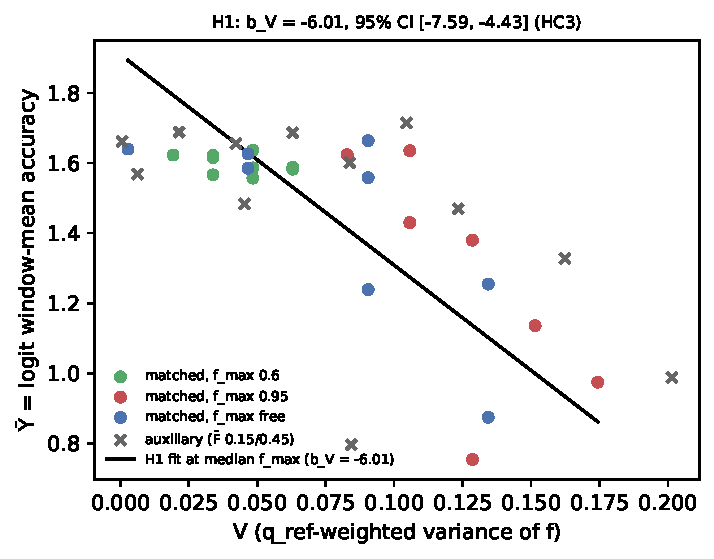
\includegraphics[width=0.62\linewidth]{../figures/out/fig_grid_h1.pdf}
\caption{Configuration-mean outcome against $V$. Matched configurations are coloured by $\fmax$ level; auxiliary configurations ($\Fbar=0.15$ or $0.45$) are crosses. Line: registered H1 fit at the median $\fmax$. Duplicated configurations plot on top of each other.}
\label{fig:h1}
\end{figure}

\subsection{Secondary outcomes and mechanism}
Mean final accuracy was \AccTmatched{} in the matched and \AccTaux{} in the auxiliary arm, from 0.408 at step 0. The registered hacking indicator (final accuracy at least 0.029 below the run's peak) fired in \NhackRuns{} of 96 runs. Figure~\ref{fig:modes} shows the mechanism the theory describes: under low-$V$ and homogeneous verifiers, the share of the most-accepted mode among errors falls during training, while under high-$V$ verifiers it rises, reaching about 0.4 of all errors in the outcome window.

The lowest outcomes come from single seeds. \NlowHighV{} matched runs from high-$V$ configurations (\NlowDistinct{} distinct trajectories once duplicates are merged, plus \NlowAux{} auxiliary run) have $Y<0.3$; no low-$V$ run does. In each, the most-accepted mode is \textsf{LEN}, accepted with probability about 0.95. Accuracy first rises with the control, peaks near step 40, then falls to \LowAccT{} while \textsf{LEN} grows to \LowLenT{} of the errors (Figure~\ref{fig:supp}b): the policy learns to produce wrong-length answers that the verifier nearly always accepts. The other seed of the same configuration did not do this within 100 steps. Within-configuration seed gaps are small in general (median \SeedGapMed{} logit) but grow with $V$ (Spearman \SeedGapRho{} in the matched arm). Higher dispersion therefore adds both a lower mean and a larger chance of a hacking episode within the horizon. Two seeds per configuration cannot estimate that chance.

\begin{figure}[t]
\centering
\begin{minipage}{0.49\linewidth}\centering
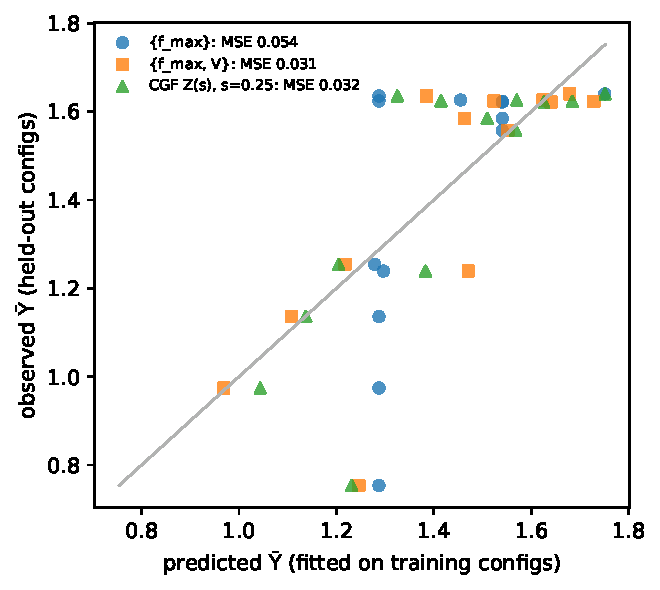
\includegraphics[width=\linewidth]{../figures/out/fig_grid_heldout.pdf}
\caption{Registered held-out comparison (H2/H3): predictions of the 13 held-out configurations from models fitted on the 23 training configurations.}
\label{fig:heldout}
\end{minipage}\hfill
\begin{minipage}{0.49\linewidth}\centering
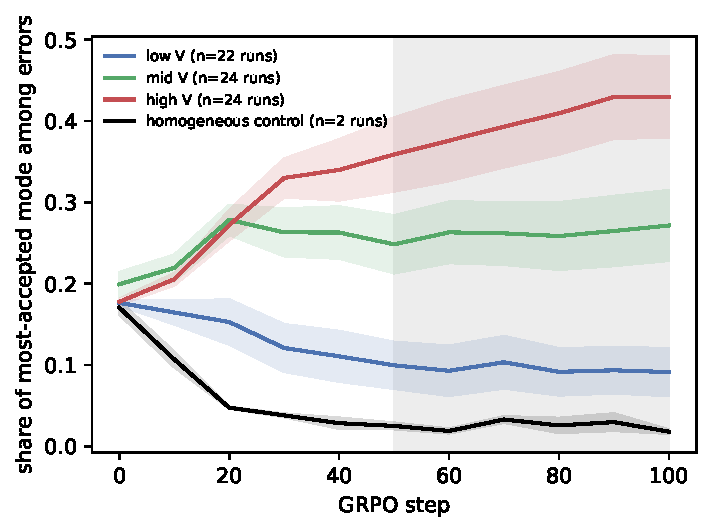
\includegraphics[width=\linewidth]{../figures/out/fig_grid_modes.pdf}
\caption{Share of each configuration's most-accepted mode among wrong answers (sampled census on 1{,}000 prompts), by $V$ tertile, matched arm, mean $\pm$ SE over runs. Shaded: outcome window.}
\label{fig:modes}
\end{minipage}
\end{figure}

\section{Aggregate verifier quality versus heterogeneity}\label{sec:aggregate}
The matched arm holds the aggregate rates fixed, so there H1 already measures dispersion beyond aggregate quality. The registered secondary analysis lets the aggregate rate vary across both arms ($n=\SecN$ configurations, $\Fbar\in\{0.15,0.3,0.45\}$, $\tau=0.9$ throughout). All comparisons in this section are labelled exploratory: they are either registered secondary analyses without a pre-specified test or, where noted, post hoc.

\textbf{Single predictors.} Leave-one-configuration-out MSE relative to the variance of $\bar Y$ (lower is better; 1.0 is no better than the mean): $V$ \RelV, $V_{q^2}$ \RelVqtwo, CGF \RelCGF, $\fmax$ \RelFmax, $\kappa_3$ \RelKappa, $\max_k q_kf_k$ \RelMaxqf, trigger frequency \RelTrig, intercept only \RelNull{} (Figure~\ref{fig:pred}). The design aggregate false-acceptance rate alone reaches \RelAggF.

\textbf{Nested models (post hoc).} Adding $\fmax$ to the aggregate rate gives \RelAggFM; adding $V$ instead gives \RelAggFV; with all three, \RelAggFMV, and the coefficient of $V$ is \AggFMVcoefV{} (CI \AggFMVcoefVLo{} to \AggFMVcoefVHi), while that of the aggregate rate is \AggFMVcoefF{} (CI \AggFMVcoefFLo{} to \AggFMVcoefFHi). On distinct verifiers only, the relative MSE is \UniqRelFM{} without and \UniqRelFMV{} with $V$, and the $V$ coefficient is \UniqAggV{} (CI \UniqAggVLo{} to \UniqAggVHi). Over this range of aggregate rates, dispersion carries more information about the outcome than the aggregate rate does.

\textbf{Registered joint model.} The registered secondary model with all estimable predictors (aggregate rate, $\fmax$, trigger frequency, $V$, $\kappa_3$, $V_{q^2}$, $\max_k q_kf_k$; $J$ and $J_{\text{worst}}$ are exact aliases of the aggregate rate and $\fmax$ when $\tau$ is constant) predicts with relative MSE \SecRel, but its predictors are highly collinear (variance inflation factor of $V$: \SecVifV), so no single coefficient is identified: $b_V=\SecV$ (CI \SecVLo{} to \SecVHi). We do not interpret its coefficients.

\textbf{Realised rate (post hoc).} The realised window false-acceptance rate alone predicts better than any design statistic (relative MSE \RelAggR; with $\fmax$ and $V$, \RelAggRMV). In H1 with the realised rate added, $b_V$ shrinks from \HoneBV{} to \MedBV{} (CI \MedBVLo{} to \MedBVHi). Because the realised rate is itself moved by $V$ (Figure~\ref{fig:supp}a), this is a mediator, not a confounder: the result is consistent with dispersion acting largely by raising the on-policy false-acceptance rate as the policy shifts toward accepted modes. It does not show that the realised rate is a usable design-time predictor, because it is only known after training.

\begin{figure}[t]
\centering
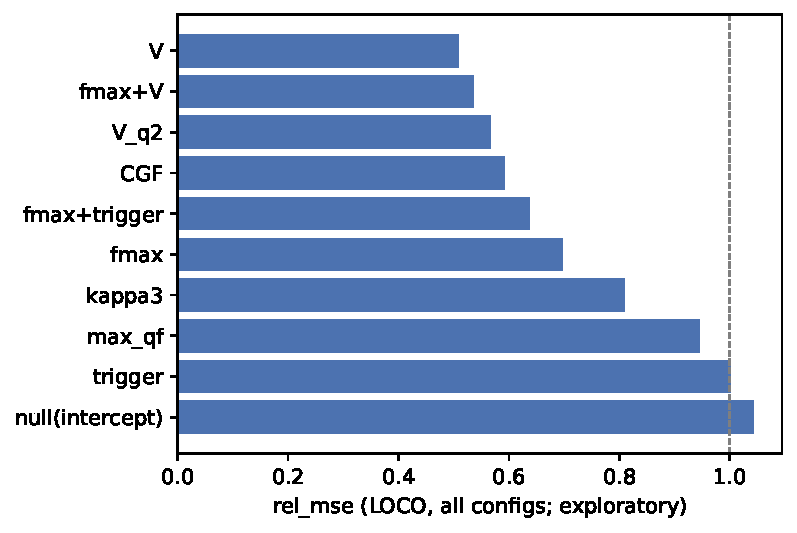
\includegraphics[width=0.5\linewidth]{../figures/out/fig_grid_predictors.pdf}
\caption{Leave-one-configuration-out MSE relative to $\operatorname{Var}(\bar Y)$ for every registered predictor set, all 48 configurations (exploratory).}
\label{fig:pred}
\end{figure}

\begin{figure}[t]
\centering
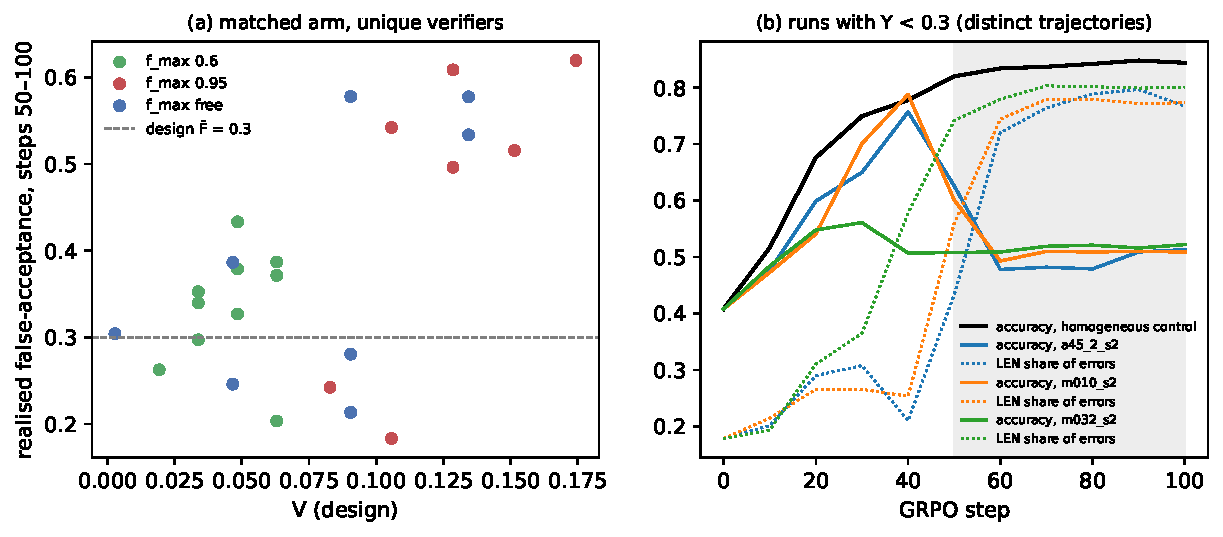
\includegraphics[width=\linewidth]{../figures/out/fig_grid_supp.pdf}
\caption{(a) Realised false-acceptance rate on wrong rollouts in the outcome window against design $V$ (matched arm, distinct verifiers). (b) Runs with $Y<0.3$: accuracy (solid) and \textsf{LEN} share of errors (dotted) against the homogeneous control. Exploratory.}
\label{fig:supp}
\end{figure}

\section{Robustness and sensitivity}\label{sec:robust}
The three registered robustness re-fits of H1 (labelled exploratory in the registration) agree with the primary estimate: without the homogeneous control $b_V=\RobNoHomBV$ (CI \RobNoHomLo{} to \RobNoHomHi); on final rather than window accuracy $b_V=\RobFinalBV$ (CI \RobFinalLo{} to \RobFinalHi); and with only configurations that have two valid seeds the fit is identical, because no run was lost. Post hoc checks:
\begin{itemize}
\item \emph{Distinct verifiers} (the duplicate disclosure above): $b_V=\UniqBV$ (CI \UniqBVLo{} to \UniqBVHi, df 22). Leave-one-verifier-out over the \NuniqueMatched{} distinct matched verifiers still favours $\{\fmax,V\}$ over $\{\fmax\}$ (MSE \UniqLooFV{} vs \UniqLooF; paired difference \UniqDiff, CI \UniqDiffLo{} to \UniqDiffHi), and the CGF is again equal to $\{\fmax,V\}$ (\UniqLooZ). On the \PureN{} registered held-out verifiers that have no twin in training, the H2 difference is \PureDiff{} (CI \PureLo{} to \PureHi): with six configurations this comparison is uninformative, and it does not reproduce the registered H2 advantage.
\item \emph{Influence}: dropping any one configuration moves $b_V$ between \LooBVmin{} and \LooBVmax.
\item \emph{Run-level model} with configuration-clustered standard errors: $b_V=\ClustBV$ (CI \ClustLo{} to \ClustHi).
\item \emph{Rank-based}: partial Spearman correlation of $\bar Y$ and $V$ given $\fmax$, \PartialSpear.
\item \emph{Hacking episodes}: removing the runs with $Y<0.3$ (a sensitivity check only; the registered estimate keeps every run) gives $b_V=\NoLowBV$ (CI \NoLowBVLo{} to \NoLowBVHi), so the association is not carried by the few hacking runs alone.
\end{itemize}
